\chapter{tirxBujAkAra saMkeyxgaLu}

oMdariMda AraMBavAguva karxmAgata saMKeyxgaLanunx kUDutAtx hoVdare baruva motatxkekx tirxBujAkAra saMkeyxgaLeMdu hesaru. I riVtiya saMKeyxgaLanunx tirxBujada rUpadalilx bareyabahudu AdadxriMdaleV I hesaru baMdide.

\begin{minipage}[c]{4cm}
\begin{flalign*}
&1=1&\\
&1+2=3\\
&1+2+3=6\\
&1+2+3+4=10\\
&1+2+3+\cdots n = \frac{n(n+1)}{2}\\
\end{flalign*}
\end{minipage}
\begin{minipage}[c]{5cm}
\text{ivugaLelalxvU {\bf tirxBujAkAra} saMKeyxgaLu}
\end{minipage}

ivugaLanunx $T(n)$ eMba cihenxyiMda sUcisutetxve.

\begin{minipage}[c]{5cm}
\begin{align*}
T(1) &= \frac{1\times 2}{2} =1\\
T(2) &= \frac{2\times 3}{2} =3\\
T(3) &= \frac{3\times 4}{2} =6\\
\end{align*}
\end{minipage}
\begin{minipage}[c]{5cm}
$\therefore T(n) = \frac{n(n+1)}{2}$
\end{minipage}

eraDu karxmAgata tirxBujAkAra saMKeyxgaLu vagaRsaMKeyxyanunxMTu mADutatx.
\begin{equation*}
\left.
\begin{aligned}
T(1)+T(2) &= 1+3 = 4\\
T(3)+T(4) &= 6+10 = 16
\end{aligned}
\qquad\right\}
\qquad\text{vagaRsaMKeyxgaLu}
\end{equation*}
\begin{align*}
T(n-1)+T(n) &= \frac{(n-1)n}{2} +\frac{n(n+1)}{2}\\
&= \frac{n^2-n+n^2+n}{n} = \frac{2n^2}{2}=n^2\\
\end{align*}

yAvudAdarU tirxBujAkArada saMkeyxya  $8$ raSaTxkekx $1$ nunx seVrisidare vagaRsaMKeyxyu pArxpatxvAgutatxde.
\begin{equation*}
\begin{aligned}
8T(1)+1 &=8+1 =9\\
8T(2)+1 &=24+1 =25\\
8T(4)+1 &=80+1 =81\\
\end{aligned}
\qquad\text{vagaRsaMKeyxgaLu}
\end{equation*}

\begin{align*}
8T(n)+1 &= \frac{8\cdot n(n+1)}{2}+1\\
&= 4n(n+1)+1\\
&=4n^2+4n+1\\
&=(2n+1)^2 \qquad \text{vagaR saMKeyx}
\end{align*}

$2\left\{100 T(n)+12\right\}+1$ eMba sUtarxvu vagaRsaMkeyxyanunx niVDutatxde.
\begin{equation*}
\begin{aligned}
n=1 \quad \text{AdAga} \quad &2\left\{100T(1)+12\right\}+1\\
       &=2\times 112+1 = 225\\[0.2cm]
n=1 \quad \text{AdAga} \quad &2\left\{100T(2)+12\right\}+1\\
       &=2\times 312+1 = 625\\[0.2cm]
n=1 \quad \text{AdAga} \quad &2\left\{100T(3)+12\right\}+1\\
 &=2\times 612+1 = 1225\\      
\end{aligned}
\qquad\text{ivelalxvU vagaRsaMKeyxgaLu}
\end{equation*}
I riVti laBayxvAda vagaRsaMKeyxgaLelalxvU $25$ ralilx konegANutatxve.
\begin{flalign*}
1^2&= 1&\\
3^2 &=1+8 =9\\
6^2 &= 1+8+27 =36\\
10^2 &= 1+8+27+64 =100
\end{flalign*}
aMdare karxmAgata tirxBujAkAra saMKeyxgaLa vagaRgaLu, karxmAgata Gana saMKeyxgaLa motatxkekx sama.

\begin{itemize}
\item[{\rm I}] tirxBujAkAra saMKeyxgaLanunx I riVti sUcisabahudu.
\begin{figure}[h]
\centering
%\includegraphics{src/figure/m_071.eps}
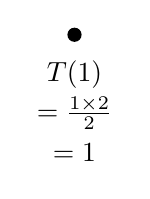
\begin{tikzpicture}[scale=0.5]%%figure-m_071
\path ( 0,0) node [shape=circle,draw,fill=black!100,scale=0.5] {}
(0,-1)node{$T(1)$}
(0,-2)node{$=\frac{1\times 2}{2}$}
(0,-3)node{$=1$};
\end{tikzpicture}
\quad
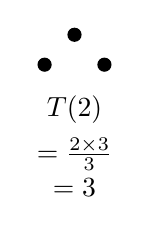
\begin{tikzpicture}[scale=0.38]
\path ( 0,2) node [shape=circle,draw,fill=black!100,scale=0.5] {}
( 1,1) node [shape=circle,draw,fill=black!100,scale=0.5] {}
(-1,1) node [shape=circle,draw,fill=black!100,scale=0.5] {}
(0,-0.5)node{$T(2)$}
(0,-2)node{$=\frac{2\times 3}{3}$}
(0,-3.1)node{$=3$};
\end{tikzpicture}
\qquad
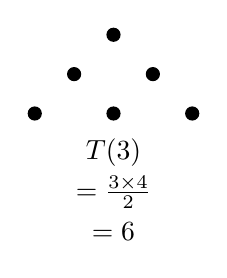
\begin{tikzpicture}[scale=0.5]
\path ( 0,2) node [shape=circle,draw,fill=black!100,scale=0.5] {}
 ( 1,1) node [shape=circle,draw,fill=black!100,scale=0.5] {}
 (-1,1) node [shape=circle,draw,fill=black!100,scale=0.5] {}
 ( 0,0) node [shape=circle,draw,fill=black!100,scale=0.5] {}
 (-2,0) node [shape=circle,draw,fill=black!100,scale=0.5] {}
 ( 2,0) node [shape=circle,draw,fill=black!100,scale=0.5] {}
  (0,-1) node {$T(3)$}
  (0,-2) node {$=\frac{3\times 4}{2}$}
  (0,-3) node {$=6$}
  ;
 \end{tikzpicture}
 \qquad
 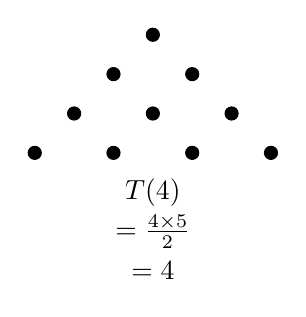
\begin{tikzpicture}[scale=0.5]
\path ( 0,2) node [shape=circle,draw,,fill=black!100,scale=0.5] {}
 ( 1,1) node [shape=circle,draw,fill=black!100,scale=0.5] {}
 (-1,1) node [shape=circle,draw,fill=black!100,scale=0.5] {}
 ( 0,0) node [shape=circle,draw,fill=black!100,scale=0.5] {}
 (-2,0) node [shape=circle,draw,fill=black!100,scale=0.5] {}
 ( 2,0) node [shape=circle,draw,fill=black!100,scale=0.5] {}
 (-3,-1) node [shape=circle,draw,fill=black!100,scale=0.5] {}
 (-1,-1) node [shape=circle,draw,fill=black!100,scale=0.5] {}
 (3,-1) node [shape=circle,draw,fill=black!100,scale=0.5] {}
 (1,-1) node [shape=circle,draw,fill=black!100,scale=0.5] {}
 (0,-2) node {$T(4)$}
 (0,-3) node {$=\frac{4\times 5}{2}$}
 (0,-4) node {$=4$};
 \end{tikzpicture}
\end{figure}
\item[{\rm II}] tirxBujAkArada saMKeyxgaLanunx I riVtiyalUlx sUcisabahudu.
\begin{figure}[h]
\centering
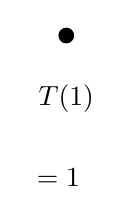
\begin{tikzpicture}%figure-m_071a
\begin{scope}
    \node[draw,fill=black!100,circle,scale=0.3] (A) at (0,1.3) {1};%%stage 1
    \node [](B) at (0,0.5){$T(1)$};%\equation
    \node [](C) at (-0.1,-0.5){$=1$};
 \end{scope}  
\end{tikzpicture}
\hspace{0.2cm}
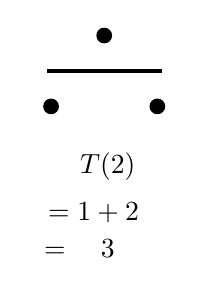
\begin{tikzpicture}[scale=0.9]
\begin{scope}
    \node[draw,fill=black!100,circle,scale=0.3] (A) at (-0.75,0.5) {1};%%stage 1
    \node[] (B) at (0.2,0) {};%path stage 1
    \node [](C) at (-1.7,0){}; 
    \node [draw,fill=black!100,circle,scale=0.3](D) at (-1.5,-0.5){4};%%stage 2
    \node [draw,fill=black!100,circle,scale=0.3](E) at (0,-0.5){5};
    \node [](D) at (-0.7,-1.35){$T(2)$};%\equation
    \node [](D) at (-0.9,-2){$=1+2$};
    \node [](D) at (-1.1,-2.5){$=\quad3$};
    \end{scope}
    \begin{scope}
     \path [line width= 1.5pt] (B) edgenode {} (C);%path stage 1
    \end{scope}    
\end{tikzpicture}
\hspace{0.2cm}
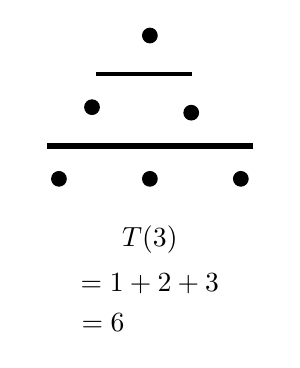
\begin{tikzpicture}[scale=0.7]
\begin{scope}
    \node[draw,fill=black!100,circle,scale=0.3] (A) at (-0.75,0.7) {1};%%stage 1
    \node[] (B) at (0.2,0) {};%path stage 1
    \node [](C) at (-1.9,0){}; 
    \node [draw,fill=black!100,circle,scale=0.3](D) at (-1.8,-0.6){4};%%stage 2
    \node [draw,fill=black!100,circle,scale=0.3](E) at (0,-0.7){5};
    \node [] (F) at (1.3,-1.3) {};%path stage 2
    \node [](G) at (-2.8,-1.3){};
    \node [draw,fill=black!100,circle,scale=0.3](H) at (-2.4,-1.9){6};%%stage 3
    \node [draw,fill=black!100,circle,scale=0.3](I) at (-0.75,-1.9){7};
    \node [draw,fill=black!100,circle,scale=0.3](J) at (0.9,-1.9){8};
    \node [](D) at (-0.75,-3){$T(3)$};%equations
    \node [](D) at (-0.75,-3.8){$=1+2+3$};
    \node [](D) at (-1.6,-4.5){$=6$};
    \end{scope}
    \begin{scope}
     \path [line width= 1.5pt] (B) edgenode {} (C);%path stage 1
     \path [line width= 2pt] (F) edgenode {} (G);%path stage 2
    \end{scope}    
\end{tikzpicture}
\hspace{0.2cm}
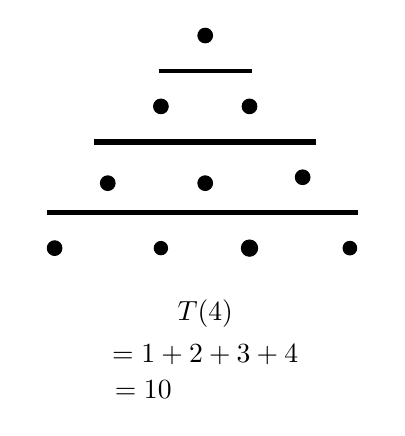
\begin{tikzpicture}[scale=0.75]
\begin{scope}
    \node[draw,fill=black!100,circle,scale=0.3] (A) at (-0.75,0.6) {1};%%stage 1
    \node[] (B) at (0.2,0) {};%path stage 1
    \node [](C) at (-1.7,0){}; 
    \node [draw,fill=black!100,circle,scale=0.3](D) at (-1.5,-0.6){4};%%stage 2
    \node [draw,fill=black!100,circle,scale=0.3](E) at (0,-0.6){5}; 
    \node [] (F) at (1.3,-1.2) {};%path stage 2
    \node [](G) at (-2.8,-1.2){}; 
    \node [draw,fill=black!100,circle,scale=0.3](H) at (-2.4,-1.9){6};%%stage 3 
    \node [draw,fill=black!100,circle,scale=0.3](I) at (-0.75,-1.9){7};
    \node [draw,fill=black!100,circle,scale=0.3](J) at (0.9,-1.8){8};
    \node [] (FF) at (2,-2.4) {};%%path stage 3
    \node [](GG) at (-3.6,-2.4){};
    \node [draw,fill=black!100,circle,scale=0.3](K) at (-3.3,-3){9};%%stage 4
    \node [draw,fill=black!100,circle,scale=0.3](L) at (-1.5,-3){a};
    \node [draw,fill=black!100,circle,scale=0.3](M) at (0,-3){A};
    \node [draw,fill=black!100,circle,scale=0.3](N) at (1.7,-3){i};
    \node [](D) at (-0.75,-4.1){$T(4)$};%equations
    \node [](D) at (-0.75,-4.8){$=1+2+3+4$};
    \node [](D) at (-1.8,-5.4){$=10$};
    \end{scope}
    \begin{scope}
     \path [line width= 1.5pt] (B) edgenode {} (C);%path stage 1
     \path [line width= 2pt] (F) edgenode {} (G);%path stage 2
     \path [line width= 2pt] (FF) edgenode {} (GG);%path stage 3
    \end{scope}    
\end{tikzpicture}
\end{figure}
\end{itemize}

